\documentclass{beamer}
\usetheme{Boadilla}
%Information to be included in the title page:
\title{Document-based Question Answering}
\author{Hachem Betrouni}
\institute{National Polytechnic school of Algiers, Industrial Engineering Department, Data Science and AI, Algiers, hachem.betrouni@g.enp.edu.dz}
\date{2023}

\AtBeginSection[]
{
  \begin{frame}
    \frametitle{Table of Contents}
    \tableofcontents[currentsection]
  \end{frame}
}

\begin{document}
\frame{
    \centering
    {\small People's Democratic Republic of Algeria}\\
    {\small Ministry of Higher Education and Scientific Research}\\
    {\small National Polytechnic School of Algiers}
    \titlepage
    \begin{tabular}{lrlcc}
        \textbf{President} & Mme. Latifa DEBBI  & Prof. & ENP,  Alger \\
        \textbf{Examiner} & Mr. Salah Eddine TACHI & MCA. & ENP,  Alger \\
        \textbf{Supervisor} & Mr. Hakim FOURAR LAIDI  & MCA. & ENP,  Alger \\
    \end{tabular}
}

\section{Introduction}
\begin{frame}
    \frametitle{Introduction}
    In today's AI consulting market, creating value goes beyond providing standard solutions. 
    The arrival of Large Language Models (LLMs) and other fundamental models raises the level of requirements. 
    To create value, bespoke AI solutions are now required, tailored to specific needs and surpassing basic requirements.
\end{frame}

\begin{frame}
    \begin{block}{The requirements}
        The requirements are no longer to predict a number, but to explain the prediction, it's no longer to recommend a blog title but to generate its whole content.
    \end{block}

    \begin{alertblock}{Market shift}
        Today we are well aware that answering individual or organizations needs for AI consulting has shifted from traditional approaches (e.g. written reports) 
        to building tangible assets that concretize the added value. Today, clients are expecting working solutions to their problems in short time.
    \end{alertblock}
\end{frame}

\section{BIGmama technology}
\begin{frame}
    \frametitle{BIGmama technology}
    \begin{figure}[h]
        \centering
        \includegraphics[width=.3\linewidth]{figures/logo.png}
    \end{figure}
    BIGmama is a French registered startup with an Algerian extension, specialized in data science and AI. 
    They have been developing predictive applications for more than 8 years.
    \begin{figure}[h]
        \centering
        \includegraphics[width=.6\linewidth]{figures/clients.png}
    \end{figure}
\end{frame}

\begin{frame}
    \begin{block}{Mission}
        BIGmama's mission is to democratize the access to bespoke AI applications, 
        With an original methodology they are able to identify, extract expertise and combine it with machine learning system 
        (Hybrid AI).
    \end{block}

    \begin{block}{Vision}
        Data science will soon become a commodity, the arrival of large language models
        mark but a start of a new wave of foundational models. 
        In the near future, we can expect the emergence of generalist models that are equivalent to ChatGPT but specialized in computer vision tasks, 
        forecasting, pattern recognition, and other domains.
    \end{block}

    \begin{exampleblock}{}
        The future is going to become in the hands of those who are capable of harnessing the power of these
        generalist models, and are capable of combining it with human expertise. 
    \end{exampleblock}
\end{frame}

\begin{frame}
    \frametitle{Unique methodology}
    \begin{block}{AI starts with \textit{problematization}}
    Problematization is going from a subject $\rightarrow$ problems. \\ 
    It's an iterative work. 
    \end{block}

    \begin{block}{AI is a tool, not an end-goal}
        Current AI approaches are not always the best way to solve \textbf{every} problem,
        certain classical approaches are more effective, simpler and more explainable to solve certain problems. 
    \end{block}

    \begin{block}{AI should be hybridized with expertise}
        By extracting expertise from our clients and combining it with AI systems, we are able to produce
        tools that are more effective, easier to maintain and that are far less expensive.
    \end{block}
\end{frame}

\begin{frame}
    \frametitle{Hyko}
    BIGmama is currently working on Hyko, a software that intrinsically embeds its mission of 
    democratizing AI and its unique methodology. 
    \begin{figure}[h]
        \centering
        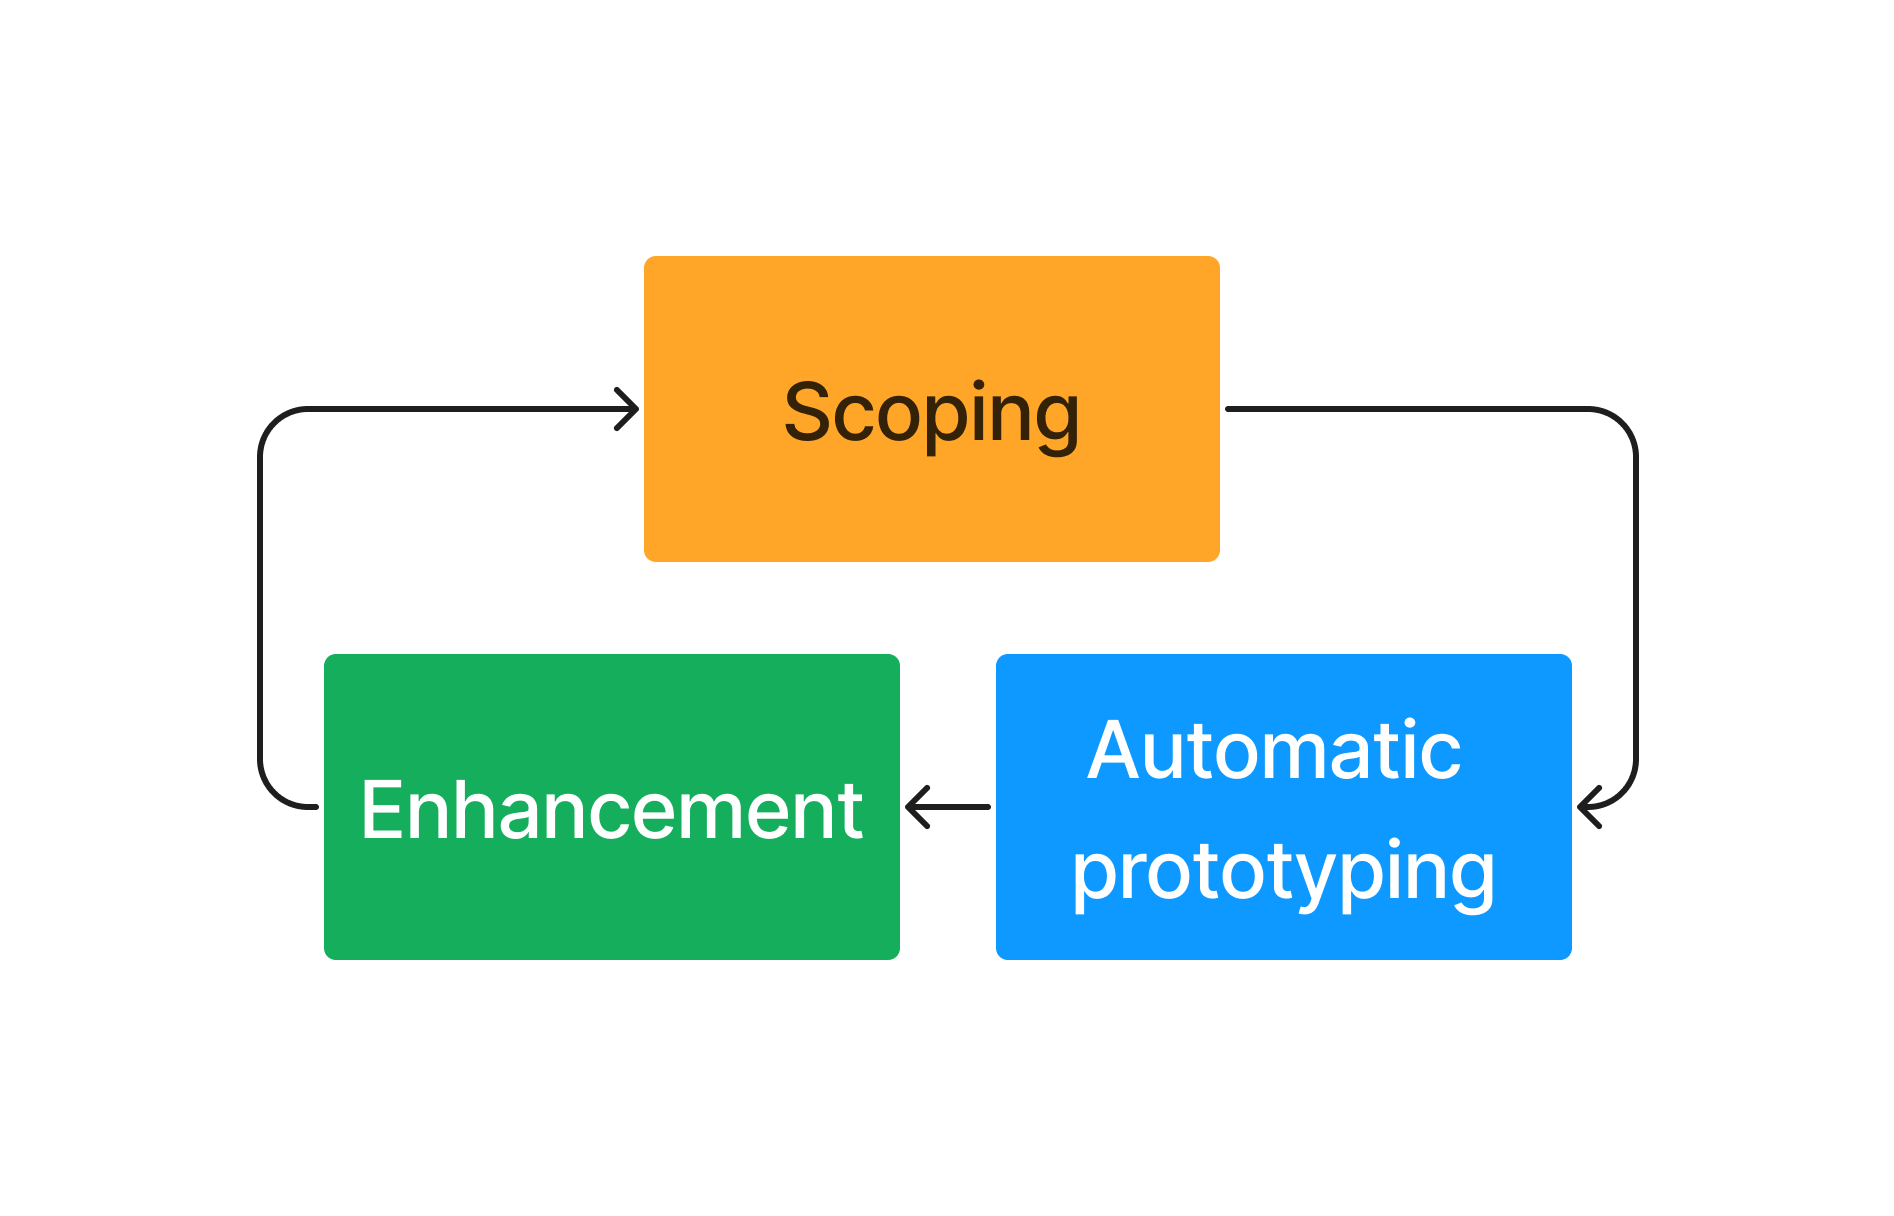
\includegraphics[width=.5\linewidth]{figures/3process.png}
        \caption{Iterative process of developing an AI asset in Hyko.}
        \label{fig:hykoprocess}
    \end{figure}
\end{frame}

\begin{frame}
    \frametitle{Hyko}
    \begin{block}{Scoping}
        
    \end{block}
    \begin{block}{Automatic prototyping}
        
    \end{block}
    \begin{block}{Prototype enhancement}
        
    \end{block}
\end{frame}

\begin{frame}{Knowledge representation}
A very important aspect of the Scoping phase is the ability to represent already existing knowledge 
(e.g. technical documents) and make it digestible by Hyko chatbot. 

\begin{figure}[h]
    \centering
    \includegraphics[width=0.5\linewidth]{figures/scopingwithdocument.png}
\end{figure}
\end{frame}


\begin{frame}{Knowledge representation}
    Previous approaches :
    \begin{itemize}
        \item Ontologies.
        \item Knowledge graphs.
    \end{itemize}
    \begin{alertblock}{}
    These methods require expertise in the targeted field, and demand careful curation of knowledge, making it an un-scalable option. 
    \end{alertblock}

    \begin{exampleblock}{}
    With the last advances in language modeling and information retrieval systems, \textbf{document-based question answering} become a more appealing option for knowledge representation.
    \end{exampleblock}
\end{frame}

\section{Document-based question answering}
\begin{frame}{Document-based question answering}
    \begin{block}{Definition}
        It's a machine learning task that focuses on extracting accurate and relevant answers from a given document and respond in natural language to a user query.
        It involves representing and manipulating content within textual documents, such as technical documentation in order to provide precise answers to user's queries.
    \end{block}

    \begin{figure}[h]
        \centering
        \includegraphics[width=\linewidth]{figures/dbqa.png}
    \end{figure}
\end{frame}

\begin{frame}{Retriever-reader}
    \begin{columns}
        \begin{column}{0.55\textwidth}
            \begin{enumerate}
                \item finding the related context in the documentation.
                \item processes the retrieved context to \textbf{extract} the start/end positions of an answer.
            \end{enumerate}
        \end{column}
        
        \begin{column}{0.45\textwidth}
            \begin{figure}[htbp]
                \centering
                \includegraphics[width=\linewidth]{figures/reader.png}
            \end{figure}
        \end{column}
    \end{columns}
\end{frame}


\begin{frame}{Retriever-generator}
    \begin{columns}
        \begin{column}{0.55\textwidth}
            Unlike the reader model, the generator model generates free text conditioned with the retrieved context to answer the question.
        \end{column}
        
        \begin{column}{0.45\textwidth}
            \begin{figure}[htbp]
                \centering
                \includegraphics[width=\linewidth]{figures/generator.png}
            \end{figure}
        \end{column}
    \end{columns}
\end{frame}

\begin{frame}{Closed-book QA}
    \begin{columns}
        \begin{column}{0.45\textwidth}
            \begin{figure}[htbp]
                \centering
                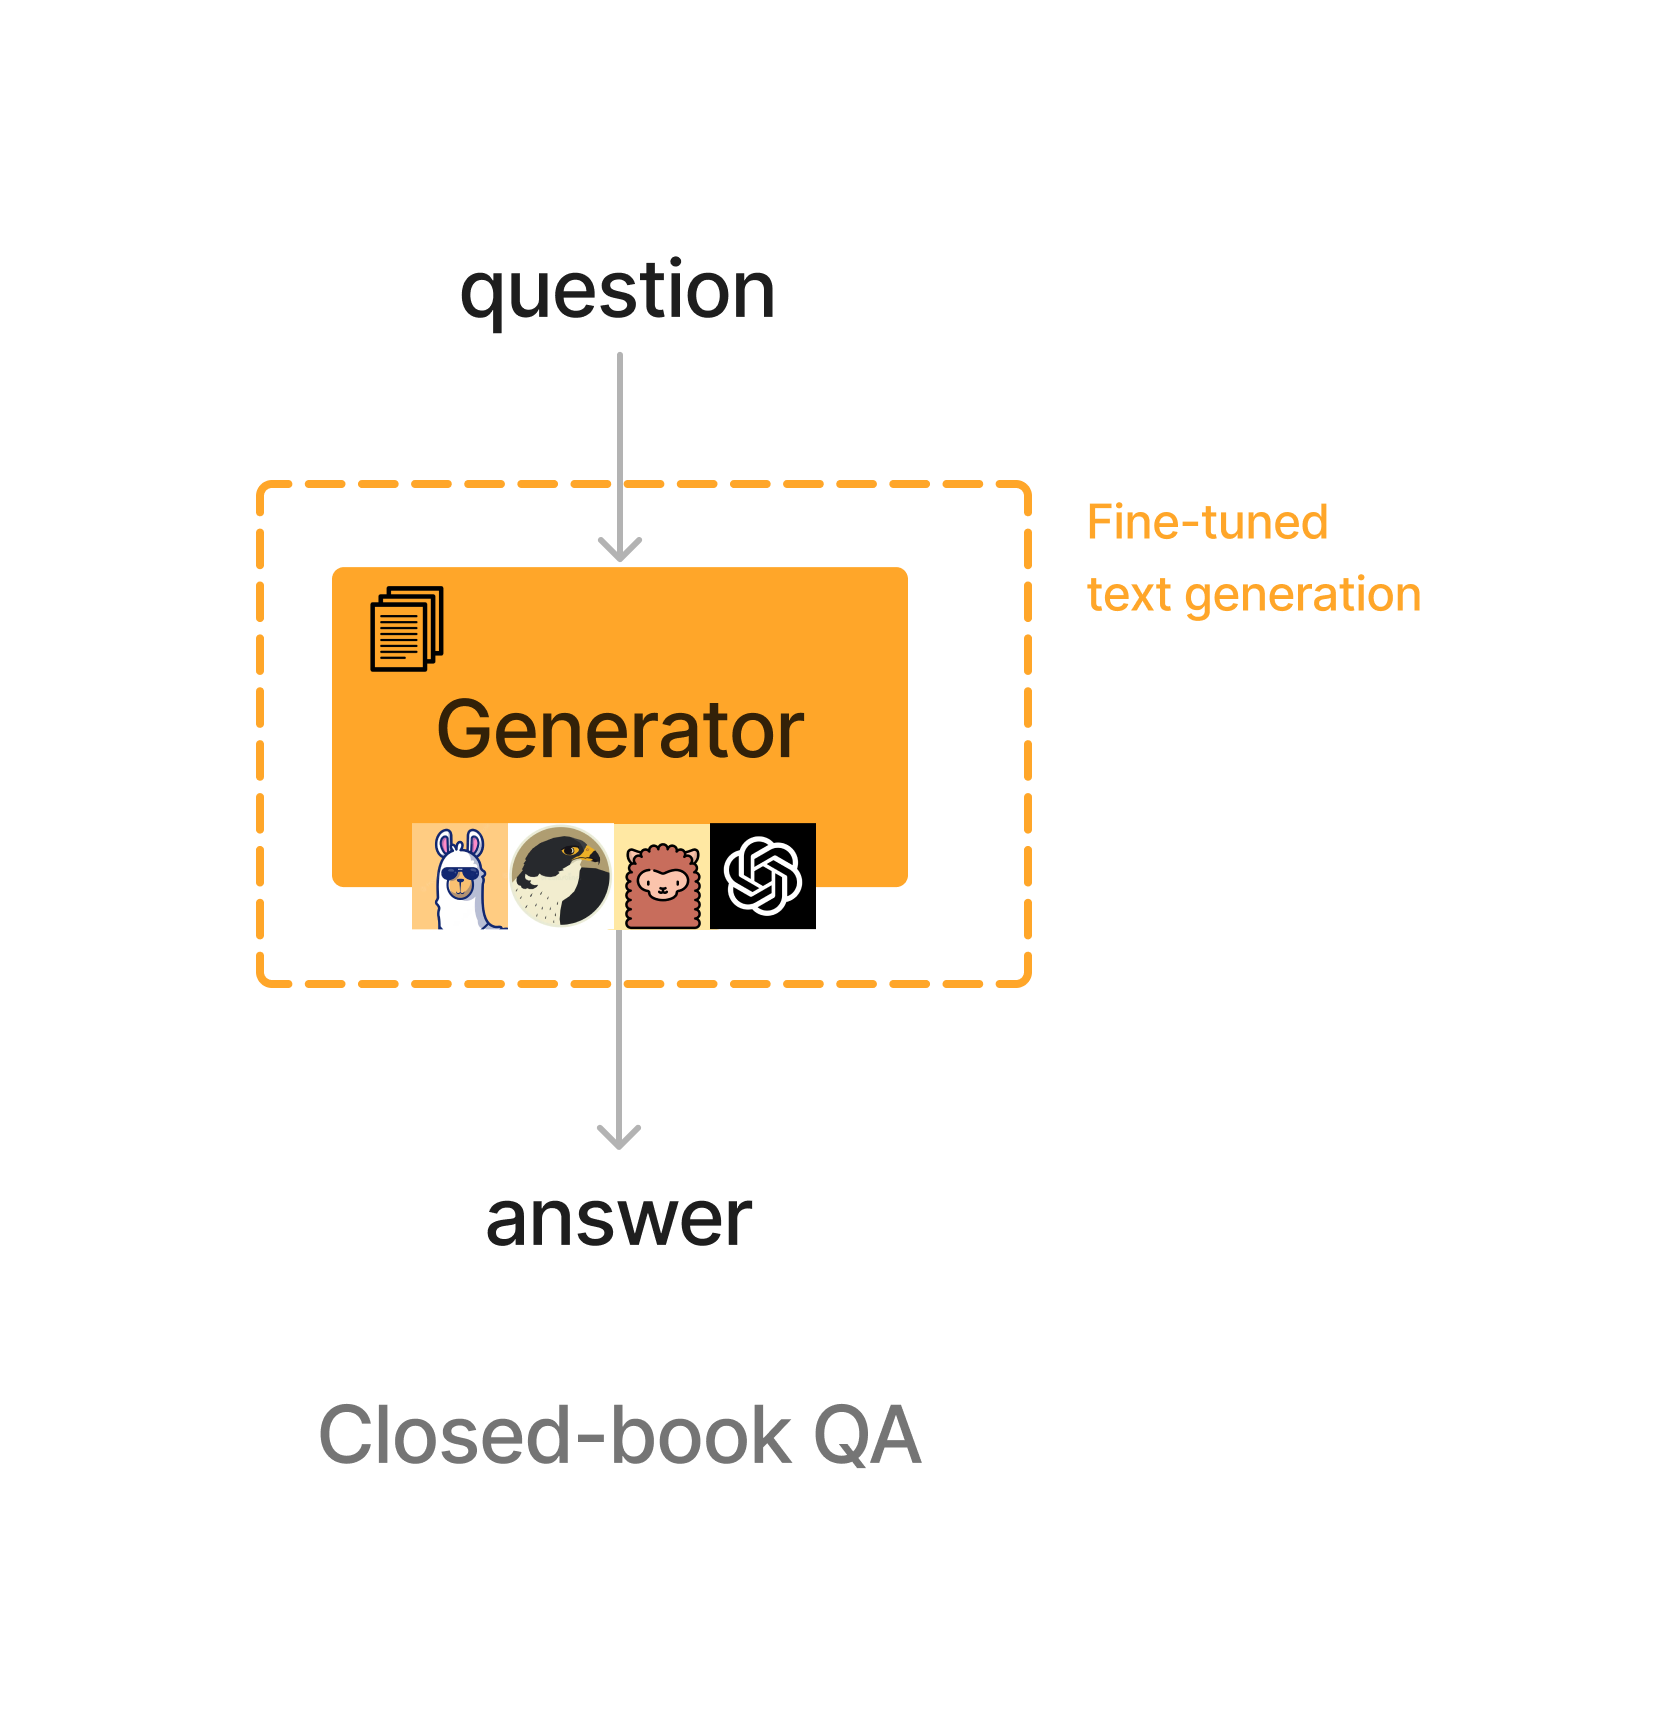
\includegraphics[width=\textwidth]{figures/closedbook.png}
            \end{figure}
        \end{column}

        \begin{column}{0.55\textwidth}
            With a substantial number of parameters, Large language models possess the ability to memorize factual information within their weight parameters. 
            Consequently, one is able to employ this property for question-answering tasks without relying on explicit context.             
        \end{column}
    \end{columns}
\end{frame}

\begin{frame}{}
    \begin{alertblock}{}
        Retriever reader models require structured data, it doesn't take advantage of unsupervised training (as LLM do).\\ 
        Closed-book approach require substantial amount of computation and time to finetune the model on new documentation.  
    \end{alertblock}

    \begin{exampleblock}{}
        Retriver-generator approach seams promising for our use-case.
    \end{exampleblock}
\end{frame}

\section{Implementation and results}
\section{Conclusion}

\end{document}